\chapter{Heap Reference Analysis}

Analyzing properties of heap data is not very trivial. This is because the spatial and temporal structure of stack and static data is simple to understand. The stack variables have a compile-time name(alias) associated with it. However, this is not the case with heap data. We need to devise a flow and context sensitive analysis to get information from heap data. 

\section{Difficulties in Analysis of Heap Data}

A program accesses data through expressions having l-values and hence are called access expressions. The l-values can either be a scalar (x), or may involve array access such as \emph{a[2*i]} or can be a reference expression like \emph{x.l.data}. In the case of reference or array, the mapping of the access expression and the l-value may change. The reference expression is primarily used to access the heap.\cite{hra} \\

Heap analysis tries to find out the answer to the questions: 
\begin{itemize}
	\item Can an access expression $a_1$ at program point $p_1$ have the same l-value as access expression $a_2$ at program  point $p_2$.
	\item Can there exist objects in the heap that will not be reachable from the access expressions?
	\item Which of the access links will be live at a particular point?
\end{itemize}
  

\section {Pointer Analysis}

Pointer analysis is a static analysis technique that establishes which pointers or heap references can point to which variables. Pointer analysis collects information about indirect accesses in programs. It can enable precise data analysis and precise inter-procedural control flow analysis. The latter will be used in the VASCO tool that will be discussed later in the report. \\

We have two types of pointer analysis information: points-to analysis and alias analysis. Alias analysis tell if two references point to the same location on the heap. It is transitive in nature. Whereas, points-to analysis tells which memory locations are pointed by references at run-time. \\

Alias information plays an important role in the liveness analysis. Must-alias information is needed to improve precision. May aliases can be found out using information from the points-to analysis. \\

In Java pointers are not created explicitly.\cite{mtpreport} All objects in Java are accessed using references and these references are termed as pointers here. Every time we create an object in Java it creates pointer to the object. This pointer could then be set to a different object or to null, but the original object will still exist. Thus points-to analysis for Java programs identifies the objects pointed to by references at run time. Thus we wish to determine
the objects pointed to by a reference variable or a field. Consider the Java program in Figure 2.1.\\

\begin{figure}
	\begin{minipage}[b]{0.45\linewidth}
		\begin{verbatim}
		
		class A(){}
		class B(){
			public A f;
			public void set(A p)
			{
				this.f = p;
			}
		}
		class C(){
		public B g;
		\end{verbatim}
	\end{minipage}
	\quad
	\begin{minipage}[b]{0.45\linewidth}
		\begin{verbatim}
		
			public void set(B q){
				this.g = q;	
			}
		}
		s1 : A x = new A()
		s2 : B y = new B()
		s3 : C z = new C()
		s4 : y.set(x);
		s5 : z.set(y);
		s5 : A a = z.g.f;
		\end{verbatim}
	\end{minipage}
	\caption{Code to illustrate heap access and points-to analysis}
\end{figure}

In the code given in Figure 2.1, three heap objects pointed to by $x$, $y$ and $z$ are created at $s_1$ , $s_2$ and $s_3$ respectively. We refer to the objects based of their allocation site as $o_1$, $o_2$ and $o_3$. The statement $s_4$ assigns the $f$ field of $o_2$ to point to $o_1$. Similarly, the $g$ field of object $o_3$ is pointed to object $o_2$. Finally the variable $a$ points to the object $o_1$, through reference field indirections.\\      

{\bfseries Liveness and Points-to Analysis} : We can remove some information from the points-to analysis result by considering only information for live pointers. For field references and indirections, liveness is defined using points-to information. \cite{liveness} \\

{\bfseries Points-to graph} in Java contain two types of edges. The first type of edge is to represent the information that reference variable $v$  is pointing to object $o$. The second type of edge represents the field $f$ of $o_1$ pointing to $o_2$. Example of points to graph for the code in Figure 2.1 is shown if Figure 2.2. \\

\begin{figure}
	\centering
	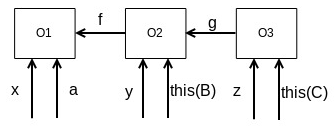
\includegraphics[width=0.6\textwidth]{Figures/rsz_points_to_graph.png}
	\caption{Points to graph for Java program in 2.1}
	\label{fig:points-to java}
\end{figure}

\section{Heap Reference Analysis}

A reference can be represented by access path. In order to perform liveness analysis of heap and identify the set of live links, naming of links is necessary. This is achieved by access path. An Access Path is defined as root variable name following any number of field names and is represented as x $\rightarrow$ n1 $\rightarrow$ n2 ....nk where x is root variable, n1 , n2 .. are field names. If access path \emph{x $\rightarrow$ f $\rightarrow$ d} is live then, the objects pointed to by \emph{x}, \emph{x.f} and \emph{x.f.d} are live. Example of access path is given for the expression \emph{x.left.right.data} in figure 2.3 \\
 
\begin{figure}
	\centering
	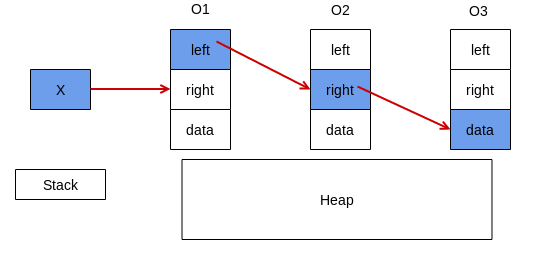
\includegraphics[width=0.6\textwidth]{Figures/hra_access_path.png}
	\caption{Heap reference using access expression \emph{x.left.right.data}.}
	\label{fig:access_path_example}
\end{figure}

An access path can be unbounded in the case of loops. Thus, we require to set a bound on the representation of access paths for liveness information. This is achieved using access graphs which summarizes information based on allocation sites. Access Graph is a directed graph representing access paths starting from root variable. Root node is connected to any number of nodes each having unique labels of form $n_i$ where n is name of the field and i is the program point. Inclusion of program points in access graphs helps in summarization and performing the merge operation.\cite{slides}
Example of access graph and liveness analysis is shown in Figure 2.4. \\

\begin{figure}
	\centering
	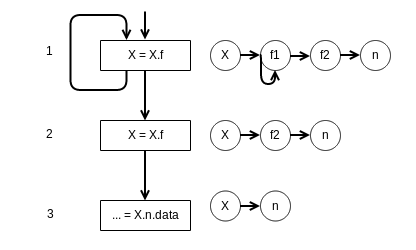
\includegraphics[width=0.6\textwidth]{Figures/heap_summarization_liveness.png}
	\caption{Example of use of access graph and liveness data flow values}
	\label{fig:access_graph_example}
\end{figure}

Availability and Anitcipability analysis of heap data : An access path $\rho$ is said to available at a program point $p$ if the target of each prefix of $\rho$ is guaranteed to be created along each path reaching $p$. An access path $\rho$ is said to be anticipable at $p$ if the target of each prefix of $\rho$ will be dereferenced along every path starting from $p$. Note that access graphs are not needed to carry out to carry out available and anticipable analysis over heap data because the sets are bounded as as result of every control flow path nature of the problems.     